\documentclass{beamer}
\usepackage{sourcecodepro}
\usepackage[english]{babel}
\usepackage[utf8]{inputenc}
\usepackage{times}
\usepackage{amsmath,amsthm, amssymb, latexsym}
\usepackage{multicol}
\usepackage{ragged2e}
\usepackage{listings}

\boldmath

\usepackage[orientation=portrait,size=a1,scale=1.6]{beamerposter}
\usetheme{LLT-poster}
\usecolortheme{ComingClean}

\title{NODAL: an Open Distributed Autotuning Library}
\author[phrb@ime.usp.br]{Pedro Bruel and Alfredo Goldman}
\institute{University of São Paulo, Brazil}
\date{\today}
\footimage{
\includegraphics[height=4cm]{usp}}

\begin{document}
\begin{frame}[fragile]
\begin{columns}[t]
    \begin{column}{.48\linewidth}
        \begin{block}{\Large Autotuning}
            \justifying
            \large
            By casting the program optimization problem as a search problem, it
            is possible to define optimization search spaces, which are usually
            very large, complex, and difficult to explore by hand.
            \begin{figure}[htpb]
                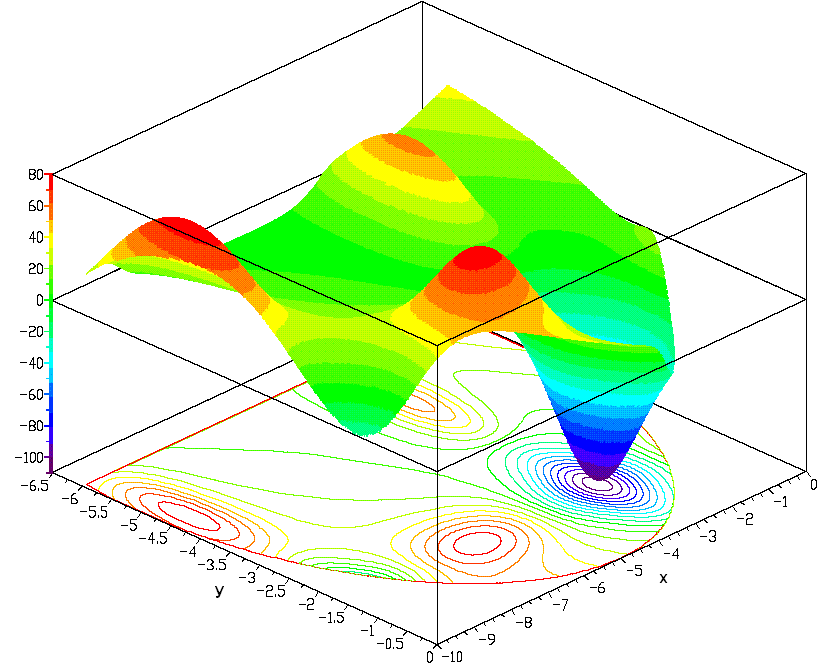
\includegraphics[width=0.6\linewidth]{sample_search_space}
                \caption{\emph{Mishra's bird function} as a sample search space}
                \label{fig:searchspace}
            \end{figure}
            The figure above illustrates what these search spaces can look
            like.  In this context, an autotuner is a tool that aids program
            optimization by automating the exploration of the optimization
            search space.
        \end{block}

        \begin{block}{\Large Example: the CUDA Compiler}
            \justifying
            \large
            An example of an autotuning problem is the selection of parameter
            values for the CUDA compiler. The figure below shows what an
            autotuner implementation for this problem should consider.
            \begin{figure}[htpb]
                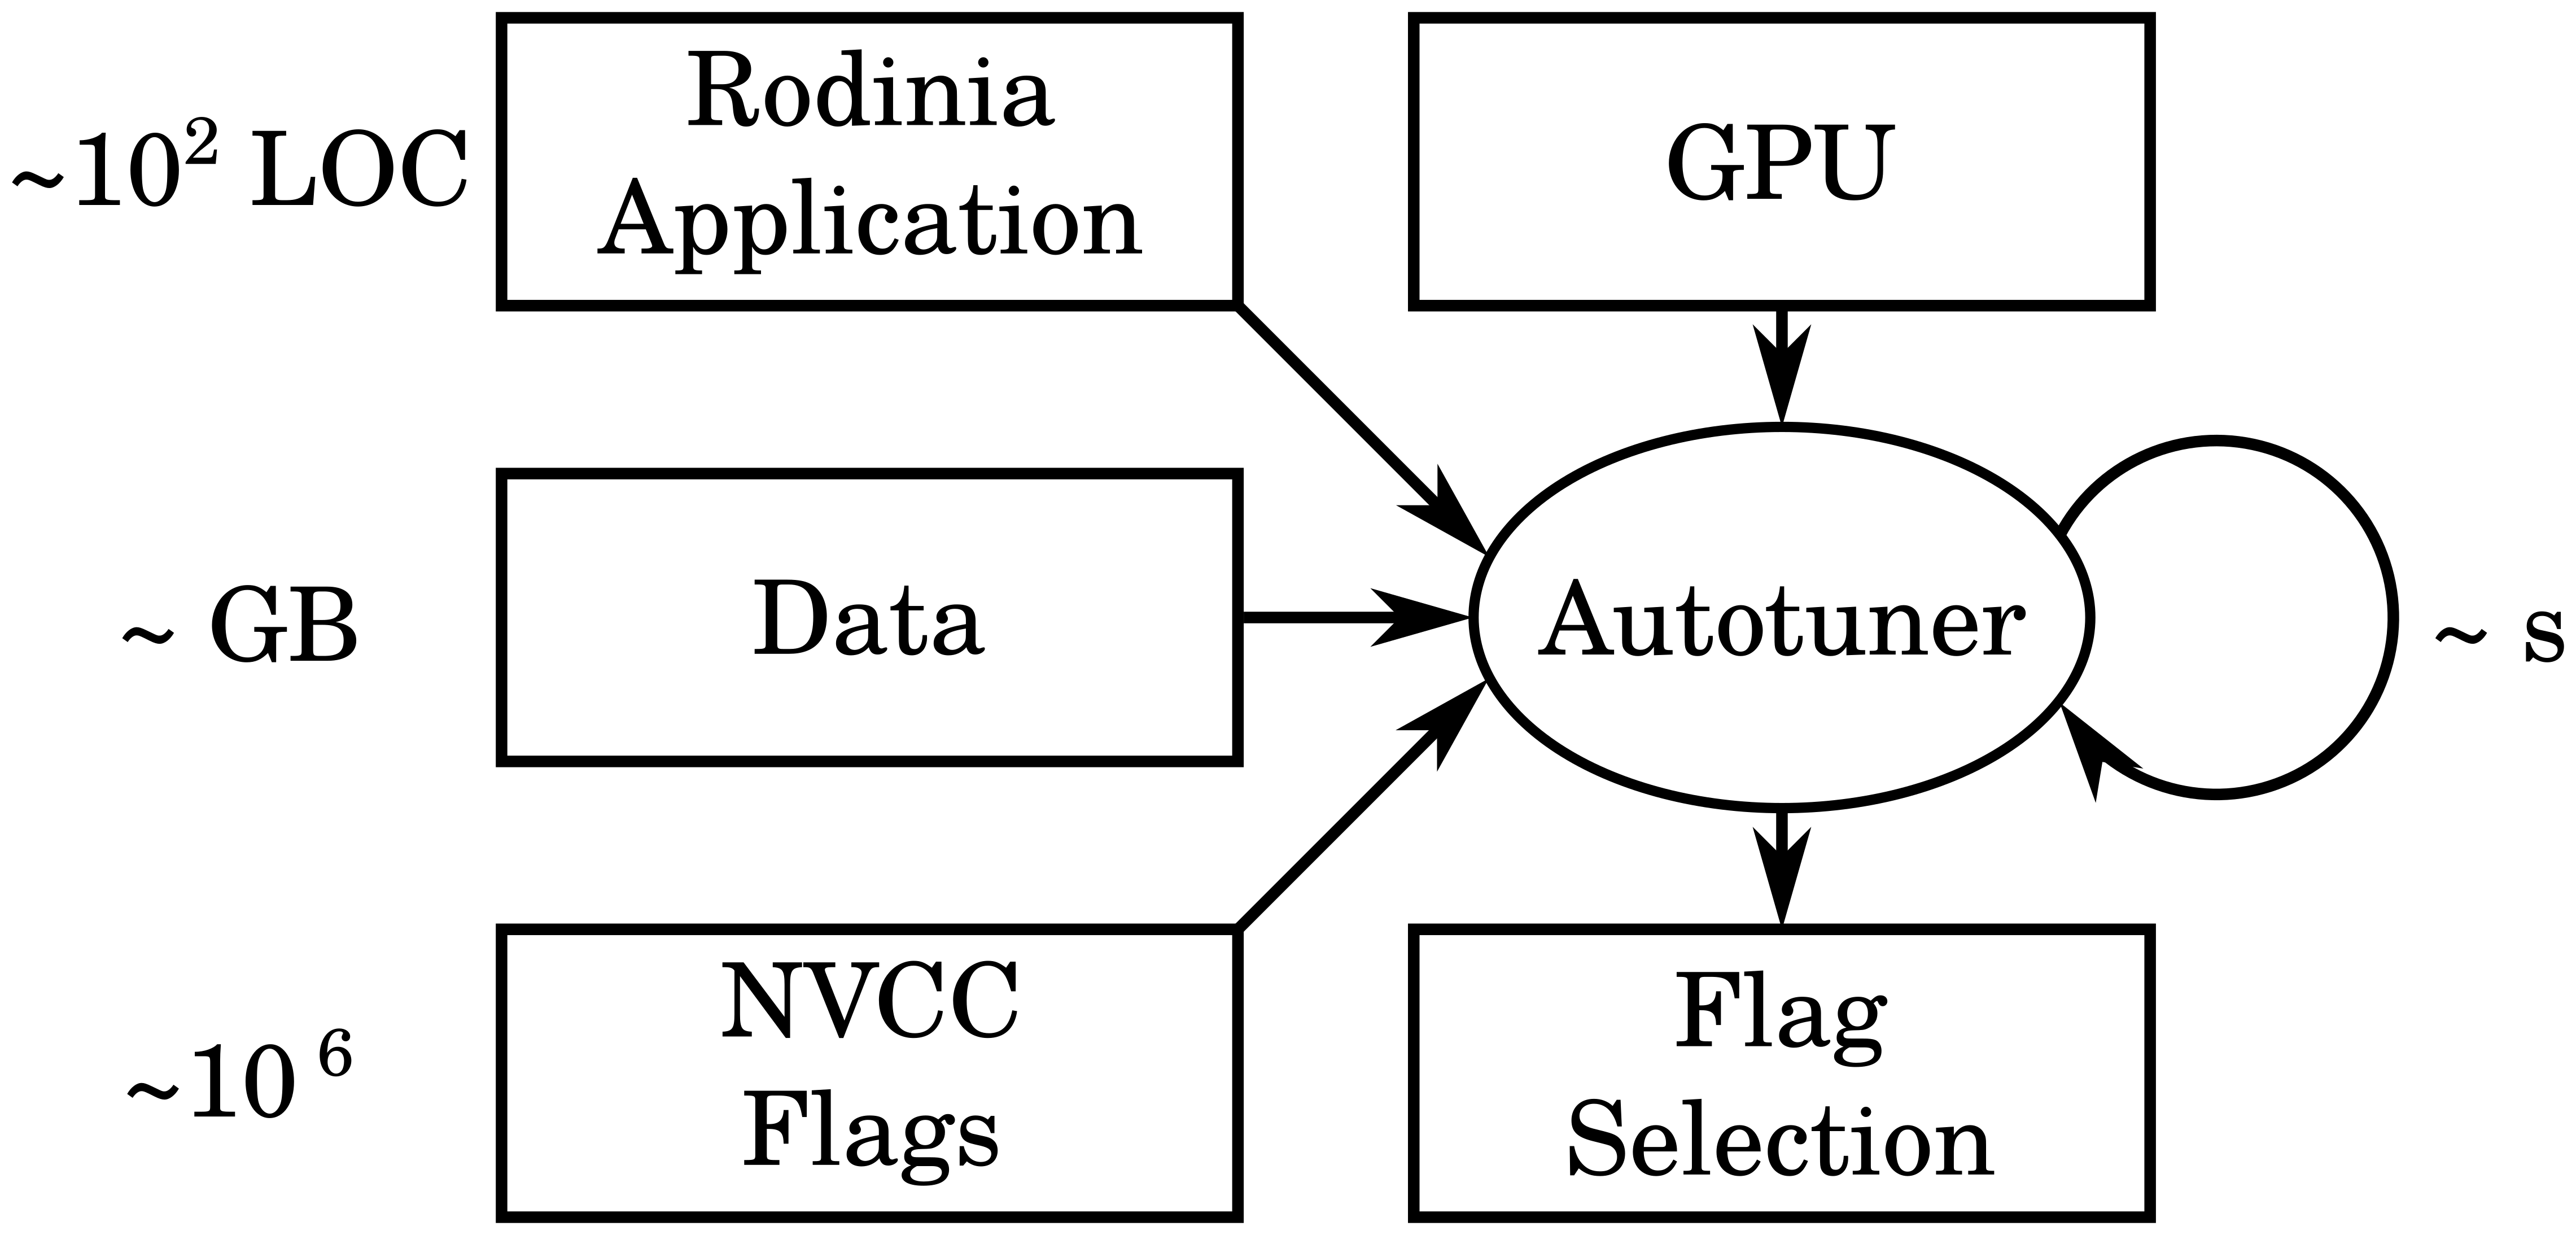
\includegraphics[width=0.95\linewidth]{overview_gpus}
            \end{figure}
            Most importantly, the autotuner should be able to explore
            efficiently the approximately $10^6$ possible parameter
            combinations.
        \end{block}

        \begin{block}{\Large Domain-Agnostic Autotuners}
            \justifying
            \large
            To autotune FPGA hardware synthesis, for example,
            one could not use the previous CUDA autotuner.
            \textbf{Domain-Agnostic Autotuners} decrease the effort of
            implementing autotuners for new domains by providing:

            \vspace{1cm}

            \begin{itemize}
                \item Abstractions for representing parameters
                \item Versatile search algorithms and strategies
                \item Mechanisms for evaluating performance metrics
            \end{itemize}
        \end{block}
    \end{column}
    \begin{column}{.48\linewidth}
        \begin{block}{\Large NODAL: Domain-Agnostic, Open, Distributed
            Autotuning using Julia}
            \justifying
            \large
            We introduce \textbf{NODAL}, an Open Distributed Autotuning Library
            in the Julia language.
            \vspace{2cm}
            \begin{figure}[htpb]
                
\includegraphics[width=0.9\linewidth]{logo}
            \end{figure}
            \vspace{2cm}

            \begin{itemize}
                \justifying\item \textbf{Domain-Agnostic:} Provides tools for representing
                    problems in multiple domains
                \justifying\item \textbf{Search:} Extensible search technique set,
                    exploration based on \emph{experimental design}
                \justifying\item \textbf{Parallel \& Distributed:} Using Julia's interfaces,
                    NODAL runs in parallel and distributed environments
            \end{itemize}
        \end{block}
        \begin{block}{\Large Try NODAL Today!}
            \justifying
            \large
            \textbf{NODAL} runs on \textbf{Julia nightly}
            and is hosted at \textbf{GitHub}:
            \vspace{2cm}
            \begin{figure}[htpb]
                
\includegraphics[width=0.2\linewidth]{github}
            \end{figure}
        \begin{lstlisting}[language=C, basicstyle=\ttfamily\large,
            numbers=none,
            frame=no, showspaces=false, showstringspaces=false,
            numberstyle=\scriptsize,
            keywords={github,com,phrb,jl},
            otherkeywords={NODAL}
        ]
        github.com/phrb/NODAL.jl
        \end{lstlisting}

            \vspace{2cm}

            \textbf{NODAL} is registered in the official Julia
            package database. To install it, run:
            \vspace{2cm}
        \begin{lstlisting}[language=C, basicstyle=\ttfamily\large,
            numbers=none,
            frame=no, showspaces=false, showstringspaces=false,
            numberstyle=\scriptsize,
            keywords={%
                @spawnat, remotecall, Nullable, Any,
                @spawn,
                @fetch, Future, Array, Float64, julia,
                while, true, function, end, put!,
                take!, sleep, RemoteChannel, Channel,
                Int, Tuple, const, addprocs, @schedule,
                @everywhere, for, in, myid, @async,
                remote_do, workers, Result, Real,
                AbstractFloat, deepcopy, rand, exp, true,
                Function, false, Run, mutable, struct,
                begin, Configuration, Dict, Symbol, using, import,
                ResultChannel, AbstractChannel, return, add, Pkg,
                NODAL%
            },
            otherkeywords={::, \&, \*, +, -, /, [, ], >, <, put!, take!,
            neighbor!, update!, NODAL}
        ]
        julia> Pkg.add("NODAL")
        \end{lstlisting}
            \vspace{2cm}
            You can try one of the examples already in the repository,
            including the CUDA compiler autotuner, and implement your own
            autotuners!
        \end{block}
    \end{column}
\end{columns}
\end{frame}
\end{document}
